\begin{wrapfigure}[25]{l}{.45\linewidth}
\vspace{-1\baselineskip}
\centerline{\includegraphics[width=.8\linewidth]{applsci-08-01039-g005-550.eps}}
\centerline{\includegraphics[width=.8\linewidth]{applsci-08-01039-g006-550.eps}}
\vspace{-1\baselineskip}
\caption{\label{fig::thomasfigs}Reproduced from Ref.~\cite{Feurer2018}. (upper) Xray pulse retrieval error increases dramatically for resolutions poorer than about 0.4\%.  
(lower) The retrieval also fails when the angular sampling falls below 8 detectors.}
\end{wrapfigure}

The technical requirements in order to achieve the pulse retrievals as needed for accuarate reconstruction are not trivial to achieve.
We are designing toward a single-shot diagnostic that reports the full temporal intensity, wavelength, and polarization distribution also with attoseconds resolution and at the highest repetition rate, up to 1MHz.  
Modeled after the original Jens Viefhaus, so called ``Cookie Box'' design, we propose a universal main chamber that accepts micro-channel plate based electron detectors in a 16-fold array.


Preliminary results of Ref.~\cite{Nick2018} were based on the original 16-fold detector array afforded 1~eV eTOF spectrometer resoltuion when working in the required single-shot current mode, not the synchrotron style high resolution counting mode.
From Fig.~\ref{fig::thomasfigs}(upper) we can see that the energy resolution for the streaked photoelectrons should ideally be in the sub~0.25\% range.
We therefore are targeting detectors that will have an energy resolution of 0.25~eV at up to 100~eV electron kinetic energy above the retardation voltage.
The retardation voltage will allow us to view even high energy electrons, including Auger electrons, with the same high resolution.
We note that the fine tuning of the sorts of novel FEL modes that allow for attosecond FEL experiments typically require a diagnostic of such 0.25~eV resolution of the spectral sub-spikes \cite{AlbertoPrivate}.

The resolution in pulse reconstruction depends also on the number of angular sample points per optical cycle.
In Fig.~\ref{fig::thomasfigs}(lower) we see a clear prescription that the angular streaking pattern should be sampled at least along 6--8 angular sample points.
The diminishing returns for adding more detector assemblies drives the design to 16 angles which is expected to provide a two-fold over-sampling of the angular dimension.
Furthermore, by shifting the dressing laser frequency toward the near-infrared we can further improve the temporal resolution.
Based on Refs.~\cite{lcls2_opportunities,Cederbaum2008,Biggs2012,Mukamel2013} we expect that much of the x-ray pulse characterization needs will lie in the sub-10 fs regime.
\begin{wrapfigure}[18]{r}{.45\linewidth}
\vspace{-0.5\baselineskip}
\centerline{\includegraphics[trim={0 0 0 0pt},width=\linewidth]{jamessim.eps}}
\vspace{-0.5\baselineskip}
\caption{\label{fig::jamessim}Simulation of two attosecond x-ray pulses separated by 4~fs dressed by a 4~$\mu$m streaking field, courtesy J.~Cryan.}
\end{wrapfigure}
We propose therefore to shift to a 2-3~$\mu$m wavelength to both improve the fractional bandwidth for a robust carrier shape and also to improve the temporal resolution while still preserving an appropriate window for pulse shape retrieval.
This change should take our initial demonstration of 500 attosecond resolution for a 10~$\mu$m, 33~fs optical cycle, angular streaking field to an expected 150 attoseconds resolution for a 3 $\mu$m field --- 11 fs optical cycle.
Figure~\ref{fig::jamessim} shows a 4~$\mu$m wavelength simulation of two xFEL pulses that are separated by only 4~fs.
By pushing further down to a 1~$\mu$m streaking field, we could expect to achieve temporal resoltuions competative with laser-based HHG state-of-the-art \cite{Zenghu2017,HJWorner2017}.

When diagnosing closely separated double pulses, the angular acceptance of the electron spectrometers are a principle concern \cite{Worner2018}.
We plan to optimize this angular acceptance such that we relax slightly the collection for the sake of preserving the resolution.
We were able to reduce the sample density by 10-fold in Ref.~\cite{Nick2018} to avoid the onset of space-charge blurring of the streaking resolution.
We expect that we can sacrifice a factor of 6 in signal in order to relax the angular collection of the eTOFs.
This reduced collection will be partially compensated by a new chamfered-pore design for the microchannel plates that improves collection efficiency.

\begin{wrapfigure}[18]{l}{.5\linewidth}
\vspace{-1\baselineskip}
\centerline{
	%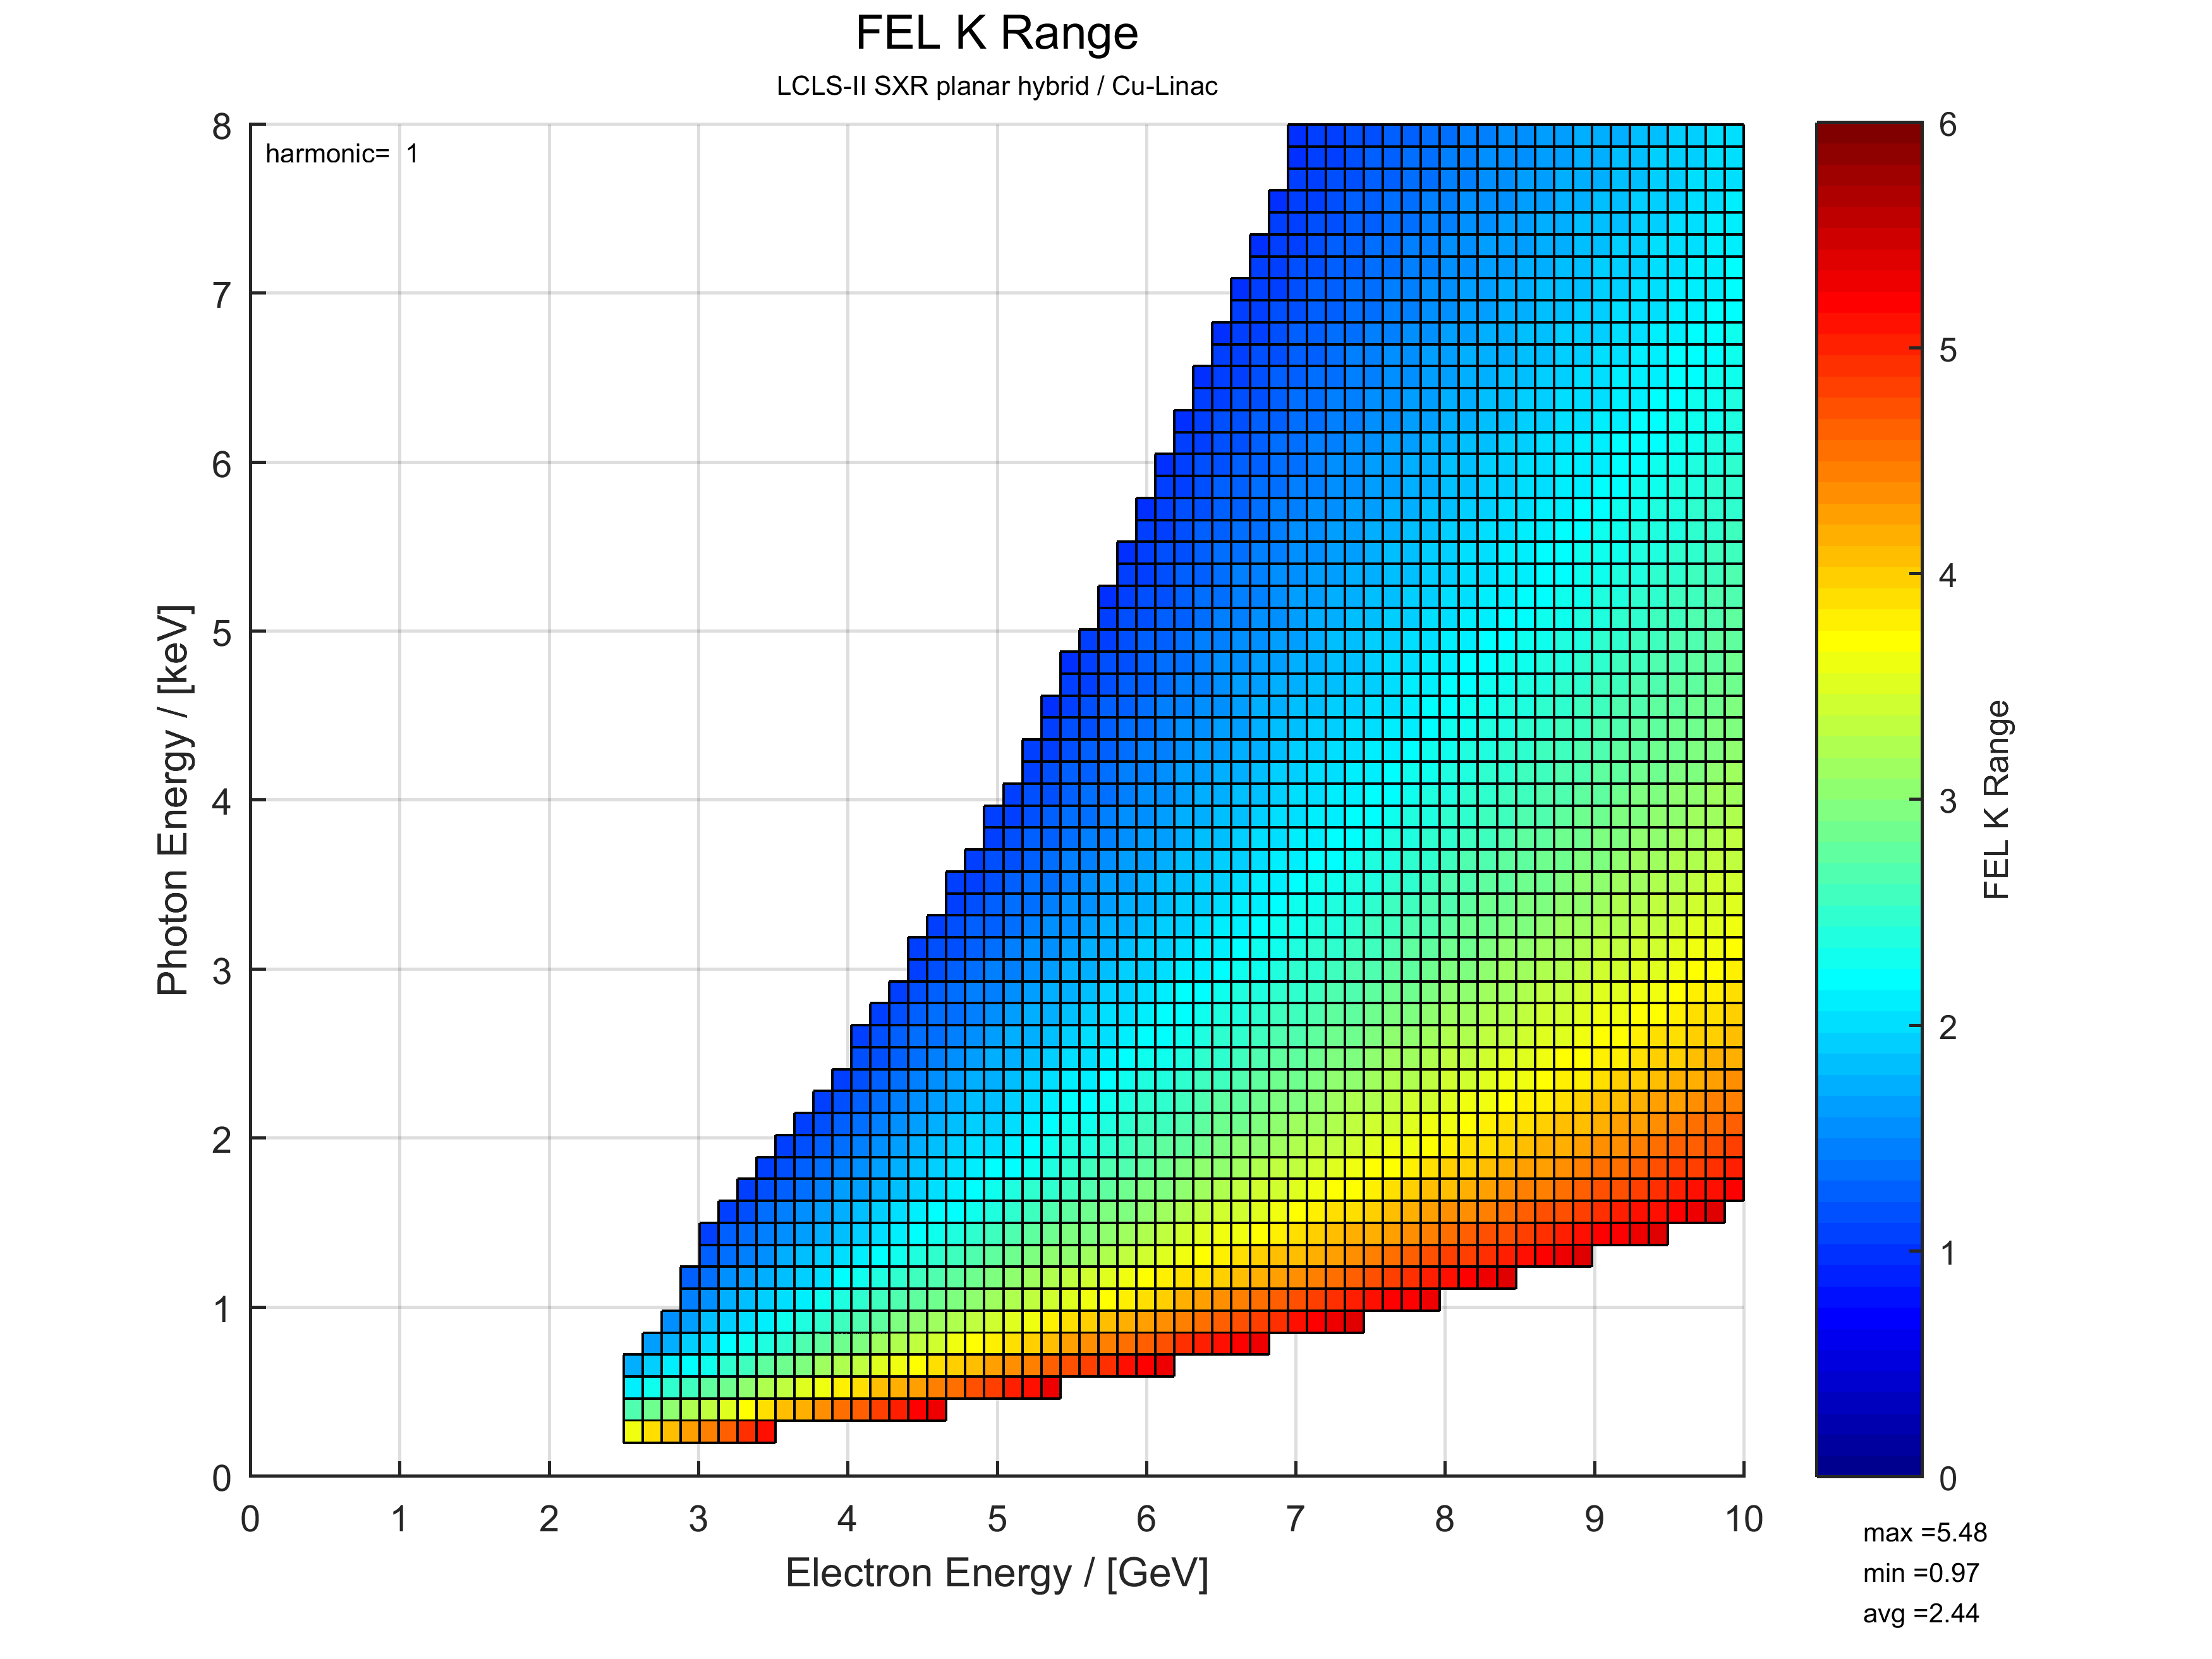
\includegraphics[width=\linewidth]{CuL_SXR_HorzPolPlanHybrid_K.eps}
	\includegraphics[width=\linewidth]{HeinzDieter_lcls2_SXU_range_lcls-tn-18-4.rangeFig.eps}
	}
\vspace{-1\baselineskip}
\caption{\label{fig::sxu_K} Soft x-ray undulator tuning range. \cite{HeinzDieter_SXU_twocolor}
	}
\end{wrapfigure}
Motivated by the great progress in multi-color FEL modes \cite{Lutman13_twocolor,Marinelli13_twocolor,Allaria2014,Marinelli2015,Prince2016,Lutman2016,Marinelli2016,Lutman2016FreshSlice}, we are capitalize on the two-fold over sampling in the angular dimension.
The color separation between multi-pulses using the new soft x-ray undulator of LCLS-II could be made to interrogate different atomic species with absorption resonances separated by hundreds of eV.
Our two-fold over sampling in the angular dimension allows us to fully retrieve the temporal, spectral, and polarization characterization of shaped multi-pulses \cite{Lutman2016,Lutman2016FreshSlice}.
Figure~\ref{fig::sxu_K} shows that the soft x-ray undulator (SXU) for LCLS-II will be capable of K values from 2 to 5 that could provide two-color pulses with one pulse below the carbon edge and the other above the oxygen edge.
We are designing for a novel configuration whereby individual detectors in the eTOF array can have vastly different retardation voltages.
We plan for tests of such a novel mode by demonstrating interleaved retardations used to measure the carbon and the oxygen Auger electron spectra simultaneously with high resolution as early as spring 2020.

Furthermore, as laser based HHG isolated attosecond pulses come available as in Refs.~\cite{Chen2014,Schmidt2016,Biegert2016,WornerSci2017} one could use a helium buffer gas to enable angular streaking simultaneously of HHG-generated EUV attosecond pulses with x-ray attosecond pulses in the identical scheme as the x-ray/x-ray pairs discussed above.
One could use the weaker HHG isolated attosecond pulses \cite{Biegert2016} as a supercontinuum probe up to the carbon K-edge.
The LCLS-II would provide the much higher power and energy attosecond pump pulses for $1s\rightarrow\mbox{valence}$ resonant pump transitions.
This would allow for strong pumping of valence electronic correlations from a chosen atomic site in the molecule well above nitrogen and oxygen, even fluorine and transition metal $L$-edges.

